\section{连续型随机变量及其分布}
\subsection{连续型随机变量及其概率密度函数}
\begin{definition}
设随机变量\(X\)的分布函数为\(F(x)\),
若存在一个非负函数\(f(x)\),
使得对任意实数\(x\),有\[
	F(x) = \int_{-\infty}^x f(t) \dd{t},
\]
则称\(X\)为\DefineConcept{连续型随机变量},
\(f(x)\)称为\(X\)的\DefineConcept{概率密度函数},
简称为\DefineConcept{密度函数}或\DefineConcept{密度}.
\end{definition}

\begin{property}\label{theorem:随机变量及其分布.连续型随机变量的密度函数的性质}
密度函数具有以下两个性质:
\begin{enumerate}
	\item 非负性:\(f(x) \geq 0, \quad x \in (-\infty,+\infty)\);
	\item 规范性:\(\int_{-\infty}^{+\infty} f(x) \dd{x} = 1\).
\end{enumerate}
\end{property}
这两个性质也是密度函数的特征,
即若任何一个函数\(g(x)\)具有以上两个性质,
则\(g(x)\)必是某一个连续型随机变量的密度函数.

\begin{theorem}
设\(X\)为连续型随机变量,\(F(x)\)和\(f(x)\)分别为\(X\)的分布函数与密度函数,则
\begin{enumerate}
	\item 对任意常数\(a < b\),有\[
		P(a < X \leq b) = \int_a^b{f(x) \dd{x}};
	\]

	\item 若\(F(x)\)是连续函数,则在\(f(x)\)的连续点\(x_0\)有\[
		F'(x_0) = f(x_0);
	\]

	\item 对任意常数\(C\),有\(P(X=C) = 0\).
\end{enumerate}
\end{theorem}

定理说明连续型随机变量取任意数值的概率都为0,即\[
	P(X=k) = 0.
\]
从而结论1可以表为\[
	P(a < X \leq b)
	= P(a \leq X \leq b)
	= P(a \leq X < b)
	= P(a < X < b)
	= \int_a^b f(x) \dd{x}.
\]
由此可见,一个连续型随机变量\(X\)的密度函数可在有限个点上取值不同,
这样并不影响\(X\)的分布函数,从而密度函数不唯一.

\subsection{常见连续型分布}

\subsubsection{均匀分布}
\begin{definition}
设随机变量\(X\)的密度函数为\begin{equation}
	f(x) = \left\{ \def\arraystretch{1.5}
	\begin{array}{cl}
		\frac{1}{b-a}, & x \in (a,b), \\
		0, & x \in (-\infty,a) \cup (b,+\infty), \\
	\end{array} \right.
\end{equation}
则称\(X\)在区间\([a,b]\)上服从\DefineConcept{均匀分布},
记为\(X \sim U(a,b)\),
其中\(a < b\).

一般地,把密度函数大于0的区间叫做连续型随机变量的取值区间.
\end{definition}

\begin{theorem}
均匀分布的分布函数为\begin{equation}
	F(x) = \left\{ \def\arraystretch{1.5}
	\begin{array}{cl}
		0, & x < a, \\
		\frac{x-a}{b-a}, & a \leq x \leq b, \\
		1, & x > b. \\
	\end{array} \right.
\end{equation}
\end{theorem}

\subsubsection{指数分布}
\begin{definition}
设随机变量\(X\)的密度函数为\begin{equation}
f(x) = \left\{ \def\arraystretch{1.5}
\begin{array}{cl}
\lambda e^{-\lambda x}, & x > 0, \\
0, & x \leq 0, \\
\end{array} \right.
\end{equation}其中\(\lambda > 0\)为常数,
则称“\(X\)服从\DefineConcept{指数分布}”,
记为\(X \sim e(\lambda)\).
\end{definition}

\begin{theorem}
指数分布的分布函数为\begin{equation}
	F(x) = \left\{ \def\arraystretch{1.5}
	\begin{array}{cl}
		1 - e^{-\lambda x}, & x > 0, \\
		0, & x \leq 0. \\
	\end{array} \right.
\end{equation}
\end{theorem}

\begin{theorem}[指数分布的无记忆性]
对于任意\(t > 0\),\(\tau > 0\),当\(X \sim e(\lambda)\)时,有\[
P(X > t + \tau \vert X > t) = P(X > \tau).
\]

指数分布是唯一具有无记忆性的连续性分布.
\end{theorem}

\subsubsection{伽马分布}
\begin{definition}
若随机变量\(X\)有密度函数\begin{equation}
	f(x) = \left\{ \def\arraystretch{1.5} \begin{array}{cl}
		\frac{\beta^\alpha}{\Gamma(\alpha)} x^{\alpha-1} e^{-\beta x},
			& x > 0, \\
		0, & x \leq 0, \\
	\end{array} \right.
\end{equation}
其中\(\alpha\)、\(\beta\)是正常数,
则称“\(X\)服从 \DefineConcept{\(\Gamma\)分布}”,
记为\(X \sim \Gamma(\alpha,\beta)\).
%@see: https://mathworld.wolfram.com/GammaDistribution.html
\end{definition}

指数分布\(e(\lambda)\)等价于\(\Gamma\)分布\(\Gamma(1,\lambda)\).

\begin{figure}[ht]
	\centering
	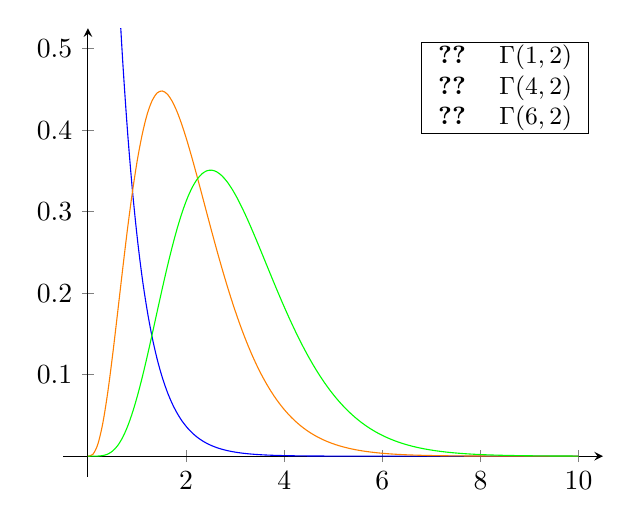
\begin{tikzpicture}
		\begin{axis}[
			name=GammaDistribution,
			axis y line=middle,
			axis x line=middle,
			enlarge x limits=0.05,
			enlarge y limits=0.05,
			ymax=.5,
			ymin=0,
		]
			\def\plotGDPDF#1#2#3{\addplot[color=#3,samples=100,smooth,domain=0:10]{%定义
				(2^(#1))*(x^(#1-1))*exp(-2*x)/(#2)
			}}%
			\plotGDPDF{1}{1}{blue};\label{pgfplots:伽马分布.Gamma(1,2)}
			\plotGDPDF{4}{6}{orange};\label{pgfplots:伽马分布.Gamma(4,2)}
			\plotGDPDF{6}{120}{green};\label{pgfplots:伽马分布.Gamma(6,2)}
		\end{axis}
		\node[draw,fill=white,inner sep=0pt,below left=0.5em]
		at(GammaDistribution.north east){\small\begin{tabular}{cl}
			\ref{pgfplots:伽马分布.Gamma(1,2)} & \(\Gamma(1,2)\) \\
			\ref{pgfplots:伽马分布.Gamma(4,2)} & \(\Gamma(4,2)\) \\
			\ref{pgfplots:伽马分布.Gamma(6,2)} & \(\Gamma(6,2)\) \\
		\end{tabular}};
	\end{tikzpicture}
	\caption{\(\Gamma\)分布的密度函数}
	% Mathematica: Plot[Table[PDF[GammaDistribution[\[Alpha], .5], x], {\[Alpha], {1, 4, 6}}] // Evaluate, {x, 0, 20}, PlotRange -> {0, .5}, Filling -> Axis]
\end{figure}


\begin{definition}
若一个元件或系统的寿命\(X\)满足一个连续型分布,\(X \sim F(t)\),
则其可靠度函数定义为\[
R(t) = 1 - F(t) = P(X > t).
\]其失效率函数定义为\[
r(t) = \frac{f(t)}{R(t)}.
\]

当\(\increment t\)较小时,\(r(t) \increment t\)表示元件或系统在时刻\(t\)以前正常工作,
但在时间\((t,t+\increment t)\)失效的概率.
\end{definition}

注意,当\(\alpha = 1\)时,\(\Gamma\)分布\(\Gamma(1,\beta)\)为指数分布\(e(\beta)\),即系统失效概率不随时间变化;
当\(0 < \alpha < 1\)时,系统失效概率随时间\(t\)增加呈下降趋势;而当\(\alpha > 1\)时则正相反.

\subsubsection{贝塔分布}
\begin{definition}
%@see: 《概率论与数理统计》(茆诗松、周纪芗、张日权) P90.
若随机变量\(X\)有密度函数\begin{equation}
	f(x) = \frac{1}{B(\alpha,\beta)} x^{\alpha-1} (1-x)^{\beta-1},
	\quad 0\leq x\leq1,
\end{equation}
其中\(\alpha,\beta\)是正常数,
\(B\)是\hyperref[equation:特殊函数.贝塔函数的定义式]{贝塔函数},
则称“\(X\)服从~\DefineConcept{\(B\)分布}”,
记为\(X \sim B(\alpha,\beta)\).
%@see: https://mathworld.wolfram.com/BetaDistribution.html
\end{definition}
